\documentclass[preprint,authoryear,12pt]{elsarticle}

\usepackage{epsfig,multirow,subfigure,amsmath,amssymb,graphicx}
\graphicspath{{./}}

\journal{ESE 545 Project Report}

\begin{document}

\begin{frontmatter}

\title{Cell SPU Lite Dual Instruction Architecture Implementation using Verilog}


\author{
Yufei Ren\\
{\small Student ID: 108006070}\\
{\small Email: yufren@ic.sunysb.edu}}

\address{Department of Electrical and Computer Engineering\\
Stony Brook University, Stony Brook, New York
}

\date{May 02, 2012}

\maketitle

\begin{abstract}

The microarchitecture of the Synergistic Processor is a
state-of-the-art architecture. Dual issue is the key character of this
architecture, which means two instruction is sent to two individual
execution pipes simutanously if there is no hazard to accelerate the
throughput of instruction. This project selects a subset of the Cell
SPU instruction set, which contains 31 common used instructions. Then
design a dual issue pipeline architecture to implement those
instructions by Verilog HDL. Test cases are also designed to test the
functionality of this implementation.

\end{abstract}

\end{frontmatter}

\section{Overview}

This project selects 31 instructions from the manual of Synergistic
Processor Unit (SPU) Instruction Set Architecture (ISA) ~\cite{sony:cellspu}. The aim of
this project is to implement this sub-instruction set by Verilog.

The first step of the project is to implement a SPU instruction
oriented parser. To translate the code in assamble language into the
format which Verilog simulator accepts, this project designs and
implements a compiler for the SPU ISA. The implementation of this
compiler will be discussed in Section~\ref{sec:compiler}.

In this project, the pipeline is divied into six modules, program
counter(PC), memory, instruction register, register file, even pipe
and odd pipe. For the even pipe, it handles fix points, floating
points and bytes computation. For the odd pipe, it handles purmute,
load and store, and branch computation. The module design will be
discussed in Section~\ref{sec:design}.

In each clock cycle, each module gets input from its precessor module
and generates output to the next module. Data signals, such as
register file contents, and control signals, such as opcode, register
file bits are transfered between modules. A global clock is used for
sychonized all the modules' timing.


\section{SPU Compiler}\label{sec:compiler}

This project implements a compiler for translate SPU assamble language
into the binary code. According to the requirement of the Verilog {\tt
  readmemh} and {\tt readmemb} function, the compiler translate the
code into hex format file and binary format file directly.

The SPU ISA defines all the instruction in the fix 32-bits width
format. The compiler gets a line from the assembler source code
file. If it gets a common instruction which is not depends on the
other lines, it translate into the object hex format string
directly. If the line is a comment line, the compiler just ignore this
line of code. In this project defination, symbols like {\tt \#}, {\tt
  ;} exists in the beginning of the source code will be treated as a
comment line. The case which the compiler has to take care of is the
{\tt branch} instruction.

Here is the C language code of the compiler implementation:

\begin{verbatim}
/* cell spu compiler */

#include <stdio.h>
#include <stdlib.h>
#include <string.h>
#include <sys/types.h>
#include <stdint.h>

static void
rmsep(char *dst, const char *src)
{
  int c;
  int srcpos, dstpos;
  int issep; /* the previous is a seperator */
  srcpos = 0;
  dstpos = 0;
  issep = 0;

  while (((c = *(src + srcpos++)) != '\0') && (c != '\n')) {
    if (c == ' ' || c == '\t' || c == ',') {
      if (issep == 0) {
        *(dst + dstpos++) = ' ';
	issep = 1;
      }
    } else {
      *(dst + dstpos++) = c;
      issep = 0;
    }
  }

  *(dst + dstpos) = '\0';

  return;
}

const char *
byte_to_binary(int x)
{
    static char b[9];
    memset(b, '\0', 9);

    int z;
    for (z = 128; z > 0; z >>= 1)
    {
        strcat(b, ((x & z) == z) ? "1" : "0");
    }

    return b;
}

static int
cellspu2hex(char *obj, const char *src)
{
  char newsrc[1024];
  memset(newsrc, '\0', 1024);

  char op[5][16];
  int i;

  uint32_t instr;

  printf("=======================\n");
  printf("original instruction is: \t%s\n", src);

  /* remove all seperator to a Space */
  rmsep(newsrc, src);

  printf("new instruction is: \t%s\n", newsrc);

  memset(&instr, '\0', 4);

  for (i = 0; i < 5; i ++) {
    memset(op[i], '\0', 16);
  }

  char *s, *e;
  s = newsrc;

  for (i = 0; (e = strchr(s, ' ')) != NULL; i ++) {
    memcpy(op[i], s, e - s);
    s = e + 1;
    printf("op[%d] = %s\n", i, op[i]);
  }
  strcpy(op[i], s);
  printf("op[%d] = %s\n", i, op[i]);

  /*  instr = op2hex(op);*/
	instr = 0;
  if (strcmp(op[0], "a") == 0) { /* Add Word */
    instr |= 0x18000000;
    instr |= atoi(op[3]) << 14;
    instr |= atoi(op[2]) << 7;
    instr |= atoi(op[1]);
  } else if (strcmp(op[0], "il") == 0) { /* immediate load word */
    instr |= 0x40800000;
    instr |= atoi(op[2]) << 7;
    instr |= atoi(op[1]);
  } else if (strcmp(op[0], "lqx") == 0) { /* load quadword x-form */
    instr |= 0x38800000;
    instr |= atoi(op[3]) << 14;
    instr |= atoi(op[2]) << 7;
    instr |= atoi(op[1]);
  } else if (strcmp(op[0], "stqx") == 0) { /* store quadword x-form */
    instr |= 0x28800000;
    instr |= atoi(op[3]) << 14;
    instr |= atoi(op[2]) << 7;
    instr |= atoi(op[1]);
  } else if (strcmp(op[0], "ah") == 0) { /* add halfword */
    instr |= 0x19000000;
    instr |= atoi(op[3]) << 14;
    instr |= atoi(op[2]) << 7;
    instr |= atoi(op[1]);
  } else if (strcmp(op[0], "ai") == 0) { /* add word immediate */
    instr |= 0x1C000000;
    instr |= atoi(op[3]) << 14;
    instr |= atoi(op[2]) << 7;
    instr |= atoi(op[1]);
  } else if (strcmp(op[0], "sf") == 0) { /* subtract from word */
    instr |= 0x08000000;
    instr |= atoi(op[3]) << 14;
    instr |= atoi(op[2]) << 7;
    instr |= atoi(op[1]);
  } else if (strcmp(op[0], "sfi") == 0) { /* subtract from word immediate */
    instr |= 0x08000000;
    instr |= atoi(op[3]) << 14;
    instr |= atoi(op[2]) << 7;
    instr |= atoi(op[1]);
  } else if (strcmp(op[0], "mpy") == 0) { /* multiply */
    instr |= 0x78800000;
    instr |= atoi(op[3]) << 14;
    instr |= atoi(op[2]) << 7;
    instr |= atoi(op[1]);
  } else if (strcmp(op[0], "mpyi") == 0) { /* multiply immediate */
    instr |= 0x74000000;
    instr |= atoi(op[3]) << 14;
    instr |= atoi(op[2]) << 7;
    instr |= atoi(op[1]);
  } else if (strcmp(op[0], "avgb") == 0) { /* average bytes */
    instr |= 0x1A600000;
    instr |= atoi(op[3]) << 14;
    instr |= atoi(op[2]) << 7;
    instr |= atoi(op[1]);
  } else if (strcmp(op[0], "avgb") == 0) { /* average bytes */
    instr |= 0x1A600000;
    instr |= atoi(op[3]) << 14;
    instr |= atoi(op[2]) << 7;
    instr |= atoi(op[1]);
  } else if (strcmp(op[0], "absdb") == 0) { /* absolute differences of bytes */
    instr |= 0x0A600000;
    instr |= atoi(op[3]) << 14;
    instr |= atoi(op[2]) << 7;
    instr |= atoi(op[1]);
  } else if (strcmp(op[0], "gbb") == 0) { /* gather bits from bytes */
    instr |= 0x36400000;
    instr |= atoi(op[2]) << 7;
    instr |= atoi(op[1]);
  } else if (strcmp(op[0], "and") == 0) { /* and */
    instr |= 0x18200000;
    instr |= atoi(op[3]) << 14;
    instr |= atoi(op[2]) << 7;
    instr |= atoi(op[1]);
  } else if (strcmp(op[0], "or") == 0) { /* or */
    instr |= 0x08200000;
    instr |= atoi(op[3]) << 14;
    instr |= atoi(op[2]) << 7;
    instr |= atoi(op[1]);
  } else if (strcmp(op[0], "xor") == 0) { /* xor */
    instr |= 0x48200000;
    instr |= atoi(op[3]) << 14;
    instr |= atoi(op[2]) << 7;
    instr |= atoi(op[1]);
  } else if (strcmp(op[0], "nand") == 0) { /* nand */
    instr |= 0x19200000;
    instr |= atoi(op[3]) << 14;
    instr |= atoi(op[2]) << 7;
    instr |= atoi(op[1]);
  } else if (strcmp(op[0], "nor") == 0) { /* nor */
    instr |= 0x09200000;
    instr |= atoi(op[3]) << 14;
    instr |= atoi(op[2]) << 7;
    instr |= atoi(op[1]);
  } else if (strcmp(op[0], "shl") == 0) { /* shift left word */
    instr |= 0x0B600000;
    instr |= atoi(op[3]) << 14;
    instr |= atoi(op[2]) << 7;
    instr |= atoi(op[1]);
  } else if (strcmp(op[0], "rot") == 0) { /* rotate word */
    instr |= 0x0B000000;
    instr |= atoi(op[3]) << 14;
    instr |= atoi(op[2]) << 7;
    instr |= atoi(op[1]);
    /*  } else if (strcmp(op[0], "br") == 0) { branch relative */
  } else if (strcmp(op[0], "bra") == 0) { /* branch absolute */
    instr |= 0x30000000;
    instr |= atoi(op[1]) << 7;
  } else if (strcmp(op[0], "brnz") == 0) { /* branch if not zero word */
    instr |= 0x21000000;
    instr |= atoi(op[2]) << 7;
    instr |= atoi(op[1]);
  } else if (strcmp(op[0], "brhnz") == 0) { /* branch if not zero word */
    instr |= 0x23000000;
    instr |= atoi(op[2]) << 7;
    instr |= atoi(op[1]);
    /*  } else if (strcmp(op[0], "hbf") == 0) { hit for branch r-form */
  } else if (strcmp(op[0], "fa") == 0) { /* floating add */
    instr |= 0x58800000;
    instr |= atoi(op[3]) << 14;
    instr |= atoi(op[2]) << 7;
    instr |= atoi(op[1]);
  } else if (strcmp(op[0], "fs") == 0) { /* floating subtract */
    instr |= 0x58A00000;
    instr |= atoi(op[3]) << 14;
    instr |= atoi(op[2]) << 7;
    instr |= atoi(op[1]);
  } else if (strcmp(op[0], "fm") == 0) { /* floating multiply */
    instr |= 0x58C00000;
    instr |= atoi(op[3]) << 14;
    instr |= atoi(op[2]) << 7;
    instr |= atoi(op[1]);
  } else if (strcmp(op[0], "fceq") == 0) { /* floating compare equal */
    instr |= 0x78400000;
    instr |= atoi(op[3]) << 14;
    instr |= atoi(op[2]) << 7;
    instr |= atoi(op[1]);
  } else if (strcmp(op[0], "fcgt") == 0) { /* floating compare greater than */
    instr |= 0x58400000;
    instr |= atoi(op[3]) << 14;
    instr |= atoi(op[2]) << 7;
    instr |= atoi(op[1]);
  } else {
    printf("unrecgonized opcode: %s\n", op[0]);
    return -1;
  }

  sprintf(obj, "%08x", instr);

  char bcode[4][9];

  memcpy(bcode[0], byte_to_binary(((instr&0xff000000)>>24)&0x00ff), 8);
  memcpy(bcode[1], byte_to_binary(((instr&0x00ff0000)>>16)&0x00ff), 8);
  memcpy(bcode[2], byte_to_binary(((instr&0x0000ff00)>>8)&0x00ff), 8);
  memcpy(bcode[3], byte_to_binary((uint32_t)(instr&0x000000ff)), 8);

  printf("%s ", bcode[0]);
  printf("%s ", bcode[1]);
  printf("%s ", bcode[2]);
  printf("%s\n", bcode[3]);

  return 0;
}

int
main(int argc, char **argv)
{

  if (argc != 3) {
    printf("Usage: scc [source file] [binary object]\n");
    exit(EXIT_FAILURE);
  }

  char src[1024], obj[1024];
  FILE *srcfp, *objfp;
  char srcbuf[1024], objbuf[1024];
  int ret;

  memset(src, '\0', 1024);
  memset(obj, '\0', 1024);
  strcpy(src, argv[1]);
  strcpy(obj, argv[2]);

  srcfp = fopen(src, "r");
  if (srcfp == NULL) {
    perror("fopen src file");
    exit(EXIT_FAILURE);
  }

  objfp = fopen(obj, "w");
  if (objfp == NULL) {
    perror("fopen obj file");
    exit(EXIT_FAILURE);
  }

  memset(srcbuf, '\0', 1024);
  memset(objbuf, '\0', 1024);
  ret = 0;
  while (fgets(srcbuf, 1024, srcfp) != NULL) {
    if ( (strlen(srcbuf) == 0) || (srcbuf[0] == '#') || (srcbuf[0] == ';') )
      continue;

    if ((ret = cellspu2hex(objbuf, srcbuf)) != 0) {
      printf("can not parse this line: \n\t%s\n", srcbuf);
      break;
    }

    fprintf(objfp, "%s\n", objbuf);
    memset(srcbuf, '\0', 1024);
    memset(objbuf, '\0', 1024);
  }

  if (ret == 0)
    printf("object file %s is created\n", obj);

  return 0;
}

\end{verbatim}


\section{Architecture Design}\label{sec:design}

The architecture issues 2 instructions in each clock cycle if there is
no hazard. To the program counter, its step is 8 instead of 4. If the
decode step finds out that there is any hazard needs to stall the
instruction execution, the program counter could be set by a signal to
indicate that the step become to 4 for structure hazard or to 0 for
data hazard (current instruction is waiting for previous instruction
to finish).

Figure ~\ref{fig:bigview} shows the overview of the
implementation. There are six modules in this implementation. We will
discuss them in detail in the following subsection.

\begin{figure}
\centering
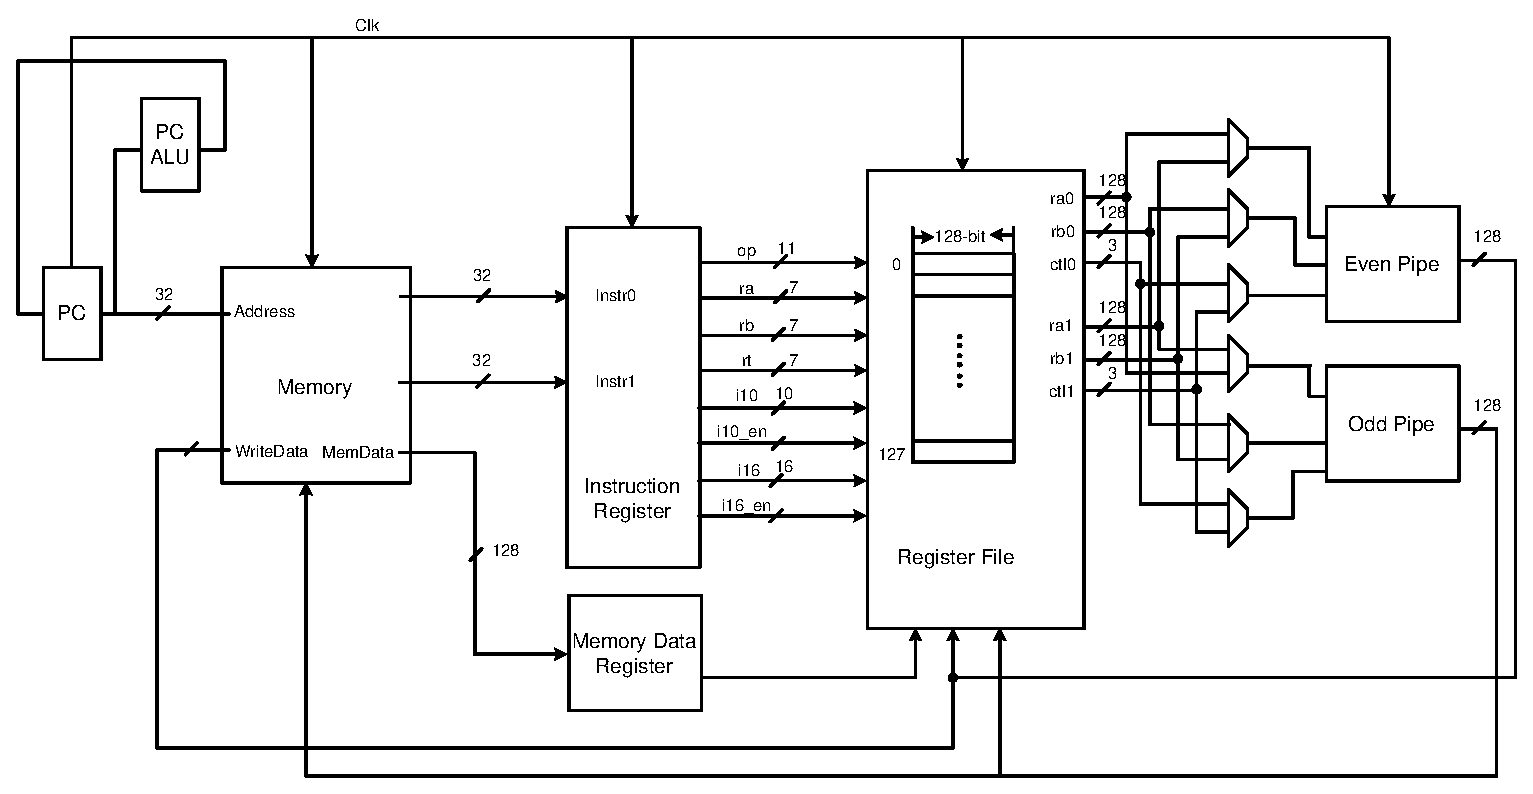
\epsfig{file=bigview.eps, width=\textwidth}
\caption{Implementation Overview}
\label{fig:bigview}
\end{figure}

There are six basic instruction formats in SPU ISA. These instructions
are all 32 bits wide. The SPU architecture defines a set of 128
general-purpose registers (GPRs), each of which contains 128 data
bits. The SPU loads and stores transfer quadwords between GPRs and local
storage.

Byte ordering defines how the bytes that make up halfwords, words,
doublewords, and quadwords are ordered in memory. The SPU supports
most-significant byte (MSB) ordering. With MSB ordering, also called
big endian, the most-significant byte is located in the lowest
addressed byte position in a storage unit (byte 0). Instructions are
described in this document as they appear in memory, with successively
higher addressed bytes appearing toward the right.

\subsection{Top Module and Cell SPU Module}

Top module is the used for connect external memory and the cell spu
module together.

\begin{verbatim}

// top level design for testing
module top #(parameter RFWIDTH = 128, WIDTH = 32, REGBITS = 7)();
   reg clk;
   reg reset;
   wire memread, memwrite;
   wire [WIDTH-1:0] adr;
   wire [WIDTH-1:0] instr0, instr1;
   wire [RFWIDTH-1:0] memdata, writedata;

   // instantiate devices to be tested
   cellspu #(RFWIDTH, WIDTH,REGBITS) spulite(clk, reset, instr0, instr1, memdata, writedata, memread, memwrite, adr);

   // external memory for instruction and data
   exmemory #(RFWIDTH, WIDTH) exmem(clk, 1, 0, 0, adr, writedata, instr0, instr1, memdata);
   
   // initialize test
   initial
     begin
        $dumpfile("top.vcd");
        $dumpvars(0,top);
	reset <= 1; # 7; reset <=0;
     end

   //generate clock to sequence tests
    always
      begin
	 clk <= 1; # 5; clk <= 0; # 5;
      end

   always@(negedge clk)
     begin
	if (memwrite)
	  if (adr == 5 & writedata == 7)
	    $display("Simulation complete successful");
	  else $display("Simulation failed");
     end
endmodule // top

\end{verbatim}

Cell SPU module contains all the modules in the following subsections
except the external memory module. In this implementation, the major
thing in the datapath which descripes the data flow, connections and
mux modules in the architecture.


\begin{verbatim}
// Yufei Ren (yufren@ic.sunysb.edu)
// Cell SPU processor - Lite edition implementation
// for ESE 545 project
module cellspu #(parameter RFWIDTH = 128, WIDTH = 32, REGBITS = 7)
             (input              clk, reset,
              input  [WIDTH-1:0] instrdata0, instrdata1,
	      input  [RFWIDTH-1:0] memdata, writedata,
              output             memread, memwrite, 
              output [WIDTH-1:0] adr);

   // wire: connect the controller and datapath
   wire [31:0] instr0, instr1;
   wire        zero, alusrca, memtoreg, iord, pcen, regwrite, regdst;
   wire [1:0]  aluop,pcsource,alusrcb;
   wire [3:0]  irwrite;
   wire [2:0]  alucont;

   // datapath
   datapath    #(RFWIDTH, WIDTH, REGBITS)
               dp(clk, reset, instrdata0, instrdata1, memdata, alusrca, memtoreg, iord, pcen,
                  regwrite, regdst, pcsource, alusrcb, irwrite, alucont,
                  zero, instr0, instr1, adr, writedata);

endmodule // cellspu

module datapath #(parameter RFWIDTH = 128, WIDTH = 32, REGBITS = 7)
                 (input              clk, reset, 
                  input  [WIDTH-1:0] memdata0, memdata1,
		  input  [RFWIDTH-1:0] memdata,
                  input              alusrca, memtoreg, iord, pcen, regwrite, regdst,
                  input  [1:0]       pcsource, alusrcb, 
                  input  [3:0]       irwrite, 
                  input  [2:0]       alucont, 
                  output             zero, 
                  output [31:0]      instr0, instr1,
                  output [WIDTH-1:0] adr,
                  output [RFWIDTH-1:0] writedata);

   localparam CONST_ZERO = 32'b0;
   localparam CONST_ONE =  32'b1;

   wire [REGBITS-1:0] ra1, ra2, wa, ra, rb, rt;
   wire [WIDTH-1:0]   pc, nextpc, rd1, rd2, wd, a, src1, src2, aluresult,
                          aluout, constx4;
   // from rf to mux
   wire [2:0] 	      cont0, cont1;
   // from mux to even pipe or odd pipe
   wire [2:0] 	      even_mode, odd_mode;
   
   wire [15:0] 	      i16_0, i16_1;
   wire [9:0] 	      i10_0, i10_1;
   wire               i10_en_0, i16_en_1;
   wire [6:0]         reg_ra_0, reg_rb_0, reg_rt_0, reg_ra_1, reg_rb_1, reg_rt_1;
   // from rf to mux
   wire [RFWIDTH-1:0]       reg_rd00, reg_rd01, reg_rd10, reg_rd11;
   // from mux to even pipe or odd pipe
   wire [RFWIDTH-1:0]       even_rd0, even_rd1, odd_rd0, odd_rd1;
   wire [RFWIDTH-1:0]       ep_result, ep_out; // even pipe result
   wire [RFWIDTH-1:0] 	    op_result, op_out; // odd pipe result
   wire [RFWIDTH-1:0] 	    md;

   wire 		    i_en_0, i_en_1, even_or_odd_0, even_or_odd_1;

   // mux selection signal
   wire                     even_mux_sel, odd_mux_sel;

   // structure hazard is determined by decode stage
   wire                     struc_hazard;
   
   mux2       #(WIDTH)  ir0(memdata0[31:0], 32'b0, 0, instr0);
   mux2       #(WIDTH)  ir1(memdata1[31:0], 32'b0, 0, instr1);
    
   // decode and check if there is any hazard
   decodeen #(WIDTH) id(clk, 1, instr0[31:0], instr1[31:0], i_en_0, i_en_1, even_or_odd_0, even_or_odd_1, reg_ra_0, reg_ra_1, reg_rb_0, reg_rb_1, reg_rt_0, reg_rt_1, i10_en_0, i10_en_1, i16_en_0, i16_en_1, i10_0, i10_1, i16_0, i16_1, struc_hazard);
   
   // datapath
   // program counter
   pcalu      #(WIDTH)  pcalu(clk, reset, 1'b1, struc_hazard, pc, nextpc);
   flopenr    #(WIDTH)  pcreg(clk, reset, 1'b1, nextpc, pc);

   // memory data register
   flop       #(RFWIDTH)  mdr(clk, memdata, md);

   // even pipe out flop
   flop       #(RFWIDTH)  epres(clk, ep_result, ep_out);
   //  odd pipe out flop
   flop       #(RFWIDTH)  opres(clk, op_result, op_out);
   
   flop       #(WIDTH)  areg(clk, rd1, a);	
//   flop       #(WIDTH)  wrd(clk, rd2, writedata);
   flop       #(WIDTH)  res(clk, aluresult, aluout);
//   mux2       #(WIDTH)  adrmux(pc, aluout, iord, adr);
   mux2       #(WIDTH)  adrmux(pc, aluout, 0, adr);
   mux2       #(WIDTH)  src1mux(pc, a, alusrca, src1);
//   mux4       #(WIDTH)  src2mux(writedata, CONST_ONE, instr[WIDTH-1:0], 
//                                constx4, alusrcb, src2);
//   mux4       #(WIDTH)  pcmux(aluresult, aluout, constx4, CONST_ZERO, pcsource, nextpc);
//   mux2       #(WIDTH)  wdmux(aluout, md, memtoreg, wd); today

   // mux for even pipe
   mux2 #(RFWIDTH) even_ra_mux(reg_rd00, reg_rd10, even_mux_sel, even_rd0);
   mux2 #(RFWIDTH) even_rb_mux(reg_rd01, reg_rd11, even_mux_sel, even_rd1);
   mux2 #(3)       even_cont_mux(cont0, cont1, even_mux_sel, even_mode);
   
   // mux for odd pipe
   mux2 #(RFWIDTH) odd_ra_mux(reg_rd00, reg_rd10, odd_mux_sel, odd_rd0);
   mux2 #(RFWIDTH) odd_rb_mux(reg_rd01, reg_rd11, odd_mux_sel, odd_rd1);
   mux2 #(3)       odd_cont_mux(cont0, cont1, odd_mux_sel, odd_mode);
   
   // register file
   regfile    #(RFWIDTH,WIDTH,REGBITS) rf(clk, regwrite, i_en_0, i_en_1, even_or_odd_0, even_or_odd_1, reg_ra_0, reg_ra_1, reg_rb_0, reg_rb_1, reg_rt_0, reg_rt_1, wa, ep_out, op_out, i10_en_0, i10_en_1, i16_en_0, i16_en_1, i10_0, i10_1, i16_0, i16_1, cont0, cont1, reg_rd00, reg_rd01, reg_rd10, reg_rd11, even_mux_sel, odd_mux_sel);

   // even pipe integer unit
   epfx       #(RFWIDTH) evenpipe(even_rd0, even_rd1, even_mode, ep_result);
   opls       #(RFWIDTH) oddpipe(odd_rd0, odd_rd1, odd_mode, op_result);

   zerodetect #(WIDTH) zd(aluresult, zero);

endmodule // datapath

module flop #(parameter WIDTH = 32)
             (input                  clk, 
              input      [WIDTH-1:0] d, 
              output reg [WIDTH-1:0] q);

   always @(posedge clk)
      q <= d;
endmodule

		   
module flopen #(parameter WIDTH = 32)
               (input                  clk, en,
                input      [WIDTH-1:0] d, 
                output reg [WIDTH-1:0] q);

   always @(posedge clk)
   //begin
      if (en) q <= d;
   //$display("%b",q);
   //$finish;
   //end
endmodule

module flopenr #(parameter WIDTH = 32)
                (input                  clk, reset, en,
                 input      [WIDTH-1:0] d, 
                 output reg [WIDTH-1:0] q);
 
//   always @(posedge clk)
   always @(*)
      if      (reset) q <= 0;
      else if (en)    q <= d;
endmodule

module pcalu #(parameter WIDTH = 32)
                (input                  clk, reset, en, str_haz,
                 input      [WIDTH-1:0] d, 
                 output reg [WIDTH-1:0] q);

   wire [WIDTH-1:0] 			nextpc;

   assign nextpc = d + 8;
   
   always @(posedge clk)
      if      (reset) q <= 0;
      else if (en)
	begin
	   if (str_haz)
	     q <= nextpc - 4;
	   else
	     q <= nextpc;
	end

endmodule

module mux2 #(parameter WIDTH = 32)
             (input  [WIDTH-1:0] d0, d1, 
              input              s, 
              output [WIDTH-1:0] y);

   assign y = s ? d1 : d0; 
endmodule

module mux4 #(parameter WIDTH = 32)
             (input      [WIDTH-1:0] d0, d1, d2, d3,
              input      [1:0]       s, 
              output reg [WIDTH-1:0] y);

   always @(*)
      case(s)
         2'b00: y <= d0;
         2'b01: y <= d1;
         2'b10: y <= d2;
         2'b11: y <= d3;
      endcase
endmodule

module epfx #(parameter WIDTH = 128)
            (input      [WIDTH-1:0] a, b, 
             input      [2:0]       alucont, 
             output reg [WIDTH-1:0] result);

   wire     [WIDTH-1:0] b2, sum, slt;

   assign b2 = alucont[2] ? ~b:b; 
   assign sum = a + b2 + alucont[2];
   // slt should be 1 if most significant bit of sum is 1
   assign slt = sum[WIDTH-1];

   always@(*)
      case(alucont[1:0])
         2'b00: result <= a & b; // asynchronize way
         2'b01: result <= a | b;
         2'b10: result <= sum;
         2'b11: result <= slt;
      endcase
endmodule

module opls #(parameter WIDTH = 128)
            (input      [WIDTH-1:0] a, b, 
             input      [2:0]       alucont, 
             output reg [WIDTH-1:0] result);

   wire     [WIDTH-1:0] slw;
   
   always@(*)
      case(alucont[1:0])
         2'b00: result <= a & b; // asynchronize way
         2'b01: result <= a | b;
	 2'b10: result <= a;
      endcase
endmodule


module zerodetect #(parameter WIDTH = 32)
                   (input [WIDTH-1:0] a, 
                    output            y);

   assign y = (a==0);
endmodule
\end{verbatim}


\subsection{Program Counter}

The programmer counter determines the address of the next instruction
in the instruction memory to be executed. It wired a 32 bits address
to the memory module.


\subsection{External Memory Module}

The instructions are all 32 bits width. The memory module defines a 16
KBytes sizes array for memory. The input includes memory read signal,
memory write signal, the address to read or write, and the data to
write. The it generates a 32 bits output signal to the instruction
register for decoding.

Figure~\ref{fig:mem} shows the external memory module.

\begin{figure}
\centering
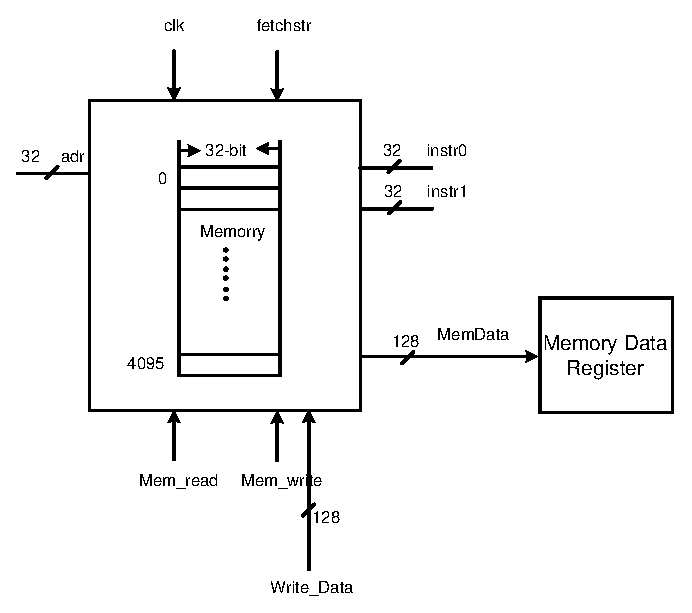
\epsfig{file=mem.eps, width=\textwidth}
\caption{External Memory Module}
\label{fig:mem}
\end{figure}


\begin{verbatim}

// external memory accessed by cellspu
// in SPU architecture, the memory means Local Storage
// in each clock cycle, the memory module send out
// for instruction, it sends out 2 * 32 bits instruction each time
// for data, it sends out 128 bits data each time
module exmemory #(parameter RFWIDTH = 128, WIDTH = 32)
   (input clk,
    input fetchinstr, memread, memwrite,
    input [WIDTH-1:0] adr,
    input [RFWIDTH-1:0] writedata,
    output reg [WIDTH-1:0] instr0, instr1,
    output reg [RFWIDTH-1:0] memdata);

   reg [31:0] 		   RAM[4095:0]; // 16KB memory array
   wire [31:0] 		   word;

   initial
     begin
	$readmemh("memoryhex.dat",RAM);
     end

   // read and write bytes from 32-bit word
   always @(posedge clk)
     begin
     if (memwrite)
       begin
	  RAM[(adr>>2)+0] <= writedata[127:96];
	  RAM[(adr>>2)+1] <= writedata[95:64];
	  RAM[(adr>>2)+2] <= writedata[63:32];
	  RAM[(adr>>2)+3] <= writedata[31:0];
       end

     if (memread)
       begin
	  memdata[127:96] <= RAM[adr>>2 + 0];
	  memdata[95:64] <= RAM[adr>>2 + 1];
	  memdata[63:32] <= RAM[adr>>2 + 2];
	  memdata[31:0] <= RAM[adr>>2 + 3];
       end
	
     if (fetchinstr)
       begin
	  instr0 <= RAM[adr>>2];
	  instr1 <= RAM[(adr>>2)+1];
       end
       // memdata <= RAM[adr>>2];
     end
   
//   assign word = RAM[adr>>2];
//   always @(*)
//     memdata <= word[31:0];  non-block mode
endmodule // exmemory

\end{verbatim}

\subsection{Instruction Register and Memory Data Register}

The instruction register has 2 32bits input ports from external
memory. Each clock cycle, it transfers 2 instrcutions from the
external memory to the instruction register.

In the Cell SPU architecture, all the registers are 128 bits
width. For the memory data register, it has a 128 bit connection from
the external meory module.

\subsection{Decode Module}

Decode module gets two instructions each clock cycle. According to the
opcode field in these two instruction, the module could determine
whether there is any structural hazard. 

The following the Decoder source codes.

\begin{verbatim}

module decodeen #(parameter WIDTH = 32)
		   (input clk, en,
		    input [WIDTH-1:0] instr0, instr1,
		    output reg i_en_0, i_en_1, even_or_odd_0, even_or_odd_1,
		    output reg [6:0] ra_0, ra_1, rb_0, rb_1, rt_0, rt_1,
		    output reg i10_en_0, i10_en_1, i16_en_0, i16_en_1,
		    output reg [9:0] i10_0, i10_1,
		    output reg [15:0] i16_0, i16_1,
                    output reg struc_hazard);

   // Even pipe execution
   parameter   EVFP    =  4'b1001;   // fix point in even pipe
   parameter   EVFX    =  4'b1010;   // float point in even pipe
   parameter   EVBY    =  4'b1011;   // byte
   // Odd pipe execution
   parameter   ODLS    =  4'b1101;   // load store
   parameter   ODPM    =  4'b1110;   // permute
   parameter   ODBR    =  4'b1111;   // branch
   
   // Instruction Opcode
   parameter   LQX     = 11'b00111000100;     // load quadword (x-form)
   parameter   STQX    = 11'b00101000100;     // store quadword (x-form)
   parameter   IL      =  9'b010000001;       // immediate load word
   parameter   ILEX    = 11'b01000000100;     // immediate load word
   parameter   AH      = 11'b00011001000;     // add halfword
   parameter   A       = 11'b00011000000;     // add word
   parameter   AI      =  8'b00011100;        // add word immediate
   parameter   AIEX    = 11'b00011100000;     // add word immediate
   parameter   SF      = 11'b00010000000;     // subtract from word
   parameter   SFI     =  8'b00001100;        // subtract from word immediate
   parameter   SFIEX   = 11'b00001100000;     // subtract from word immediate
   parameter   MPY     = 11'b01111000100;     // multiply
   parameter   MPYI    =  8'b01110100;        // multiply immediate
   parameter   MPYIEX  = 11'b01110100000;     // multiply immediate
   parameter   AVGB    = 11'b00011010011;     // average bytes
   parameter   ABSDB   = 11'b00001010011;     // absolute differences of bytes
   parameter   GBB     = 11'b00110110010;     // gather bits from bytes
   parameter   AND     = 11'b00011000001;     // and
   parameter   OR      = 11'b00001000001;     // or
   parameter   XOR     = 11'b01001000001;     // exclusive or
   parameter   NAND    = 11'b00011001001;     // nand
   parameter   NOR     = 11'b00001001001;     // nor
   parameter   SHL     = 11'b00001011011;     // shift left word
   parameter   ROT     = 11'b00001011000;     // rotate word

   parameter   BR      =  9'b001100100;       // branch relative
   parameter   BREX    = 11'b00110010000;       // branch relative
   parameter   BRA     =  9'b001100000;       // branch absolute
   parameter   BRNZ    =  9'b001000010;       // branch if not zero word
   parameter   BRHNZ   =  9'b001000110;       // branch if not zero halfword
   parameter   HBR     = 11'b00110101100;     // hint for branch (r-form)

   parameter   FA      = 11'b01011000100;     // floating add
   parameter   FS      = 11'b01011000101;     // floating subtract
   parameter   FM      = 11'b01011000110;     // floating multiply
   parameter   FCEQ    = 11'b01111000010;     // floating compare equal
   parameter   FCGT    = 11'b01011000010;     // floating compare greater than

   reg	[10:0]	    newop0, newop1;

   always @(posedge clk)
      if (en)
      begin
	 i16_en_0 <= 0;
	 i16_en_1 <= 0;
	 i10_en_0 <= 0;
	 i10_en_1 <= 0;

         i_en_0 <= 1; // the previous instruction would execute first
         i_en_1 <= 0; // if no hazard, the next instruction could execute follows by
         even_or_odd_0 <= 0;
         even_or_odd_1 <= 1;

	 struc_hazard <= 0;

	 newop0 <= 11'b0;
	 newop1 <= 11'b0;
	 	 
	 // extend 8 bits and 9 bits opcode into 11 bits opcode
	 case(instr0[31:24])
	   AI:    newop0 <= {AI, 3'b0};
	   SFI:   newop0 <= {SFI, 3'b0};
	   MPYI:  newop0 <= {MPYI, 3'b0};
	   default: begin
	      case(instr0[31:23])
	        IL: begin
                  newop0 <= {IL, 2'b0};
                  assign even_or_odd_0 = 1;
		end
	      default: begin
		 case(instr0[31:21])
		   A: assign even_or_odd_0 = 0;
		 endcase // case (instr1[31:21])
	      end
	      endcase // case (instr0[31:23])
	   end
	 endcase // case (instr0[31:24])
	 
	 case(instr1[31:24])
	   AI:    newop1 <= {AI, 3'b0};
	   SFI:   newop1 <= {SFI, 3'b0};
	   MPYI:  newop1 <= {MPYI, 3'b0};
	   default: begin
	      case(instr1[31:23])
	        IL: begin
                  newop1 <= {IL, 2'b0};
                  assign even_or_odd_1 = 1;
		end
	      default: begin
		 case(instr1[31:21])
		   A: assign even_or_odd_1 = 0;
		 endcase // case (instr1[31:21])
	      end
	      endcase // case (instr1[31:23])
	      end
	 endcase // case (instr0[31:24])
	 
	 case(instr0[31:23])
	   IL: begin 
              assign newop0 = {IL, 2'b0};
              even_or_odd_0 <= 1;
	      end
	   BR:    newop0 <= {BR, 2'b0};
	   BRA:   newop0 <= {BRA, 2'b0};
	   default: newop0 <= instr0[31:21];
	 endcase // case (instr0[31:23])
	 case(instr1[31:23])
	   IL:   begin 
              assign newop0 = {IL, 2'b0};
              even_or_odd_0 <= 1;
	      end
	   BR:    newop1 <= {BR, 2'b0};
	   BRA:   newop1 <= {BRA, 2'b0};
	   default: newop1 <= instr1[31:21];
	 endcase // case (instr0[31:23])

	 // decode the two instruction to be executed in odd pipe or even pipe, to determine if there is structure hazard
	 case(newop0)
           AH: even_or_odd_0 <= 0;
           A: even_or_odd_0 <= 0;
           AIEX: even_or_odd_0 <= 0;
           SF: even_or_odd_0 <= 0;  
           SFIEX: even_or_odd_0 <= 0;
           MPY: even_or_odd_0 <= 0;
           MPYIEX: even_or_odd_0 <= 0;
           AVGB: even_or_odd_0 <= 0;
           ABSDB: even_or_odd_0 <= 0;
           GBB: even_or_odd_0 <= 0;  
           AND: even_or_odd_0 <= 0;
           OR: even_or_odd_0 <= 0;
           XOR: even_or_odd_0 <= 0;
           NAND: even_or_odd_0 <= 0;
           NOR: even_or_odd_0 <= 0;
           FA: even_or_odd_0 <= 0;
           FS: even_or_odd_0 <= 0;
           FM: even_or_odd_0 <= 0;
           FCEQ: even_or_odd_0 <= 0;
           FCGT: even_or_odd_0 <= 0;
// odd pipe
	   ILEX: even_or_odd_0 <= 1;
           LQX: even_or_odd_0 <= 1;
           STQX: even_or_odd_0 <= 1;
           SHL: even_or_odd_0 <= 1;
           ROT: even_or_odd_0 <= 1;
           BREX: even_or_odd_0 <= 1;
           HBR: even_or_odd_0 <= 1;
	 endcase // case (newop0)
	 case(newop1)
           AH: even_or_odd_1 <= 0;
           A: even_or_odd_1 <= 0;
           AIEX: even_or_odd_1 <= 0;
           SF: even_or_odd_1 <= 0;  
           SFIEX: even_or_odd_1 <= 0;
           MPY: even_or_odd_1 <= 0;
           MPYIEX: even_or_odd_1 <= 0;
           AVGB: even_or_odd_1 <= 0;
           ABSDB: even_or_odd_1 <= 0;
           GBB: even_or_odd_1 <= 0;  
           AND: even_or_odd_1 <= 0;
           OR: even_or_odd_1 <= 0;
           XOR: even_or_odd_1 <= 0;
           NAND: even_or_odd_1 <= 0;
           NOR: even_or_odd_1 <= 0;
           FA: even_or_odd_1 <= 0;
           FS: even_or_odd_1 <= 0;
           FM: even_or_odd_1 <= 0;
           FCEQ: even_or_odd_1 <= 0;
           FCGT: even_or_odd_1 <= 0;
// odd pipe
	   ILEX: even_or_odd_1 <= 1;
           LQX: even_or_odd_1 <= 1;
           STQX: even_or_odd_1 <= 1;
           SHL: even_or_odd_1 <= 1;
           ROT: even_or_odd_1 <= 1;
           BREX: even_or_odd_1 <= 1;
           HBR: even_or_odd_1 <= 1;
	 endcase // case (newop0)

	 // structure hazard, pc += 4 instead of pc += 8
	 if (even_or_odd_0 == even_or_odd_1)
	   begin
	      i_en_0 <= 1;
	      i_en_1 <= 0;
	      struc_hazard <= 0;
	   end
	 else // no structure hazard
	   begin
	      i_en_0 <= 1;
	      i_en_1 <= 1;
	   end
	 
	 
      // decode instr0	 
	// 9 bit instruction decode
         case(instr0[31:23])
            IL:
	       begin
	          rt_0 <= instr0[6:0];
	          i16_0 <= instr0[22:7];
	          i16_en_0 <= 1;
	       end
	 endcase // case (instr[31:23])
         case(instr1[31:23])
            IL:
	       begin
	          rt_1 <= instr1[6:0];
	          i16_1 <= instr1[22:7];
	          i16_en_1 <= 1;

                  i_en_1 <= 1;
	       end
	 endcase // case (instr[31:23])

        // 11 bit instruction decode	
	case(instr0[31:21])
          A:
            begin
               ra_0 <= instr0[20:14];
               rb_0 <= instr0[13:7];
               rt_0 <= instr0[6:0];
            end
	endcase // case (instr[31:21])
	case(instr1[31:21])
          A:
            begin
               ra_1 <= instr1[20:14];
               rb_1 <= instr1[13:7];
               rt_1 <= instr1[6:0];

               i_en_1 <= 1;
            end
	endcase // case (instr[31:21])
      end
endmodule // decode

\end{verbatim}


\subsection{Register File}

The architecture has 128 global purpose registers (GPRs) in total and
all the registers are 128 bits wide. The implementation of the
register files are shown as follows.

\begin{verbatim}

// cell spu register file
module regfile #(parameter RFWIDTH = 128, WIDTH = 32, REGBITS = 7)
                (input                clk, 
                 input                regwrite,
		 input  i_en_0, i_en_1, even_or_odd_0, even_or_odd_1,
                 input  [REGBITS-1:0] ra_0, ra_1, rb_0, rb_1, rt_0, rt_1, wa,
                 input  [RFWIDTH-1:0] wd_even, wd_odd,
		 input                i10_en_0, i10_en_1, i16_en_0, i16_en_1,
                 input  [9:0]         i10_0, i10_1,
		 input  [15:0]        i16_0, i16_1,
		 output reg [2:0]     cont0, cont1,
                 output [RFWIDTH-1:0]   rd00, rd01, rd10, rd11,
                 output even_mux_sel, odd_mux_sel);

   // 128 bits * 128 GPRs
   reg  [RFWIDTH-1:0] RAM [127:0];
   wire	[RFWIDTH-1:0]	    imm0, imm1;

   // previous instruction rt
   reg [6:0] 	    pre_rt_even, pre_rt_odd;
   
   assign imm0 = {112'b0, i16_0};
   assign imm1 = {112'b0, i16_1};

   // three ported register file
   // read two ports combinationally
   // write third port on rising edge of clock
   // register 0 hardwired to 0
   always @(posedge clk)
     begin
	if (i16_en_0)
	  begin
	     RAM[rt_0] <= imm0;
	     $display("load imm0 %d into reg %d", imm0, rt_0);
	  end

	if (i16_en_1)
	  begin
	     RAM[rt_1] <= imm1;
	     $display("load imm1 %d into reg %d", imm1, rt_1);
	  end
	
        // if (regwrite) RAM[wa] <= wd;

	cont0 <= 3'b010;
	cont1 <= 3'b010;

	if (~wd_even[127]) RAM[pre_rt_even] = wd_even;
	if (~wd_odd[127]) RAM[pre_rt_odd] = wd_odd;

	pre_rt_even = rt_0;
	pre_rt_odd = rt_1;
     end

     // first instruction output
     assign rd00 = ra_0 ? RAM[ra_0] : 0;
     assign rd01 = rb_0 ? RAM[rb_0] : 0;
     assign even_mux_sel = 0;
   
     // second instruction output
     assign rd10 = ra_1 ? RAM[ra_1] : 0;
     assign rd11 = rb_1 ? RAM[rb_1] : 0;
     assign odd_mux_sel = 1;

endmodule

\end{verbatim}

\subsection{Even Pipe and Odd Pipe}

Even pipe is responsible for dealing with floating point, fix point
and byte type calculation. This project implements the fix point function shown as follows.

\begin{verbatim}

module epfx #(parameter WIDTH = 128)
            (input      [WIDTH-1:0] a, b, 
             input      [2:0]       alucont, 
             output reg [WIDTH-1:0] result);

   wire     [WIDTH-1:0] b2, sum, slt;

   assign b2 = alucont[2] ? ~b:b; 
   assign sum = a + b2 + alucont[2];
   // slt should be 1 if most significant bit of sum is 1
   assign slt = sum[WIDTH-1];

   always@(*)
      case(alucont[1:0])
         2'b00: result <= a & b; // asynchronize way
         2'b01: result <= a | b;
         2'b10: result <= sum;
         2'b11: result <= slt;
      endcase
endmodule

module opls #(parameter WIDTH = 128)
            (input      [WIDTH-1:0] a, b, 
             input      [2:0]       alucont, 
             output reg [WIDTH-1:0] result);

   wire     [WIDTH-1:0] slw;
   
   always@(*)
      case(alucont[1:0])
         2'b00: result <= a & b; // asynchronize way
         2'b01: result <= a | b;
	 2'b10: result <= a;
      endcase
endmodule

\end{verbatim}

\section{Strutural Hazard and Data Hazard}

There are two types of hazards in this architecture, structural
hazard and data hazard.

The hazard could be detected in the decode stage. For example, if
these two instructions will be issued into the same pipe, say even
pipe, there would be structure hazard in the execution stage. In this
case, the decoder sends a signal to the program counter alu that the
next clock cycle, the step becomes to 4 instead of 8.

In the decode module, it checks whether the two instructions goes into
the same pipe in the executing stage. If ture, it enables the
struc\_hazard signal to indicate the program counter to change the
step size.

\begin{verbatim}

	 // structure hazard, pc += 4 instead of pc += 8
	 if (even_or_odd_0 == even_or_odd_1)
	   begin
	      i_en_0 <= 1;
	      i_en_1 <= 0;
	      struc_hazard <= 1;
	   end
	 else // no structure hazard
	   begin
	      i_en_0 <= 1;
	      i_en_1 <= 1;
	   end
\end{verbatim}

Once the program counter alu gets the struc\_hazard signal, it changes the step size from 8 to 4.

\begin{verbatim}

   always @(posedge clk)
      if      (reset) q <= 0;
      else if (en)
	begin
	   if (str_haz)
	     q <= nextpc - 4;
	   else
	     q <= nextpc;
	end

\end{verbatim}

\section{Test results}

In this section, the project designs a series of test cases to show
the functionality of the implementation. The test environment is in
Fedora 14 linux operation system. The verilog code is compiled by the
iverilog (Icarus Verilog compiler), and the runtime engine is vvp
(Icarus Verilog runtime engine).

The project use GTK Wave to view the sequence and value changes in the
time sequence.

\subsection{Load immediate and Add}

This test loads immediate data into register file first, and then add
the contents of these two registers into another register.

Assamble file:

\begin{verbatim}
il	2,5
il	2,5
il	3,10
il	3,10
a	10,3,2
il	4,10
a	10,3,2
il	5,2
a	10,10,4
\end{verbatim}

hex file is:

\begin{verbatim}
40800282
40800282
40800503
40800503
1800818a
40800504
1800818a
40800105
1801050a
\end{verbatim}


Figure~\ref{fig:test_fig1} shows the illustration of this test.

\begin{figure}
\centering
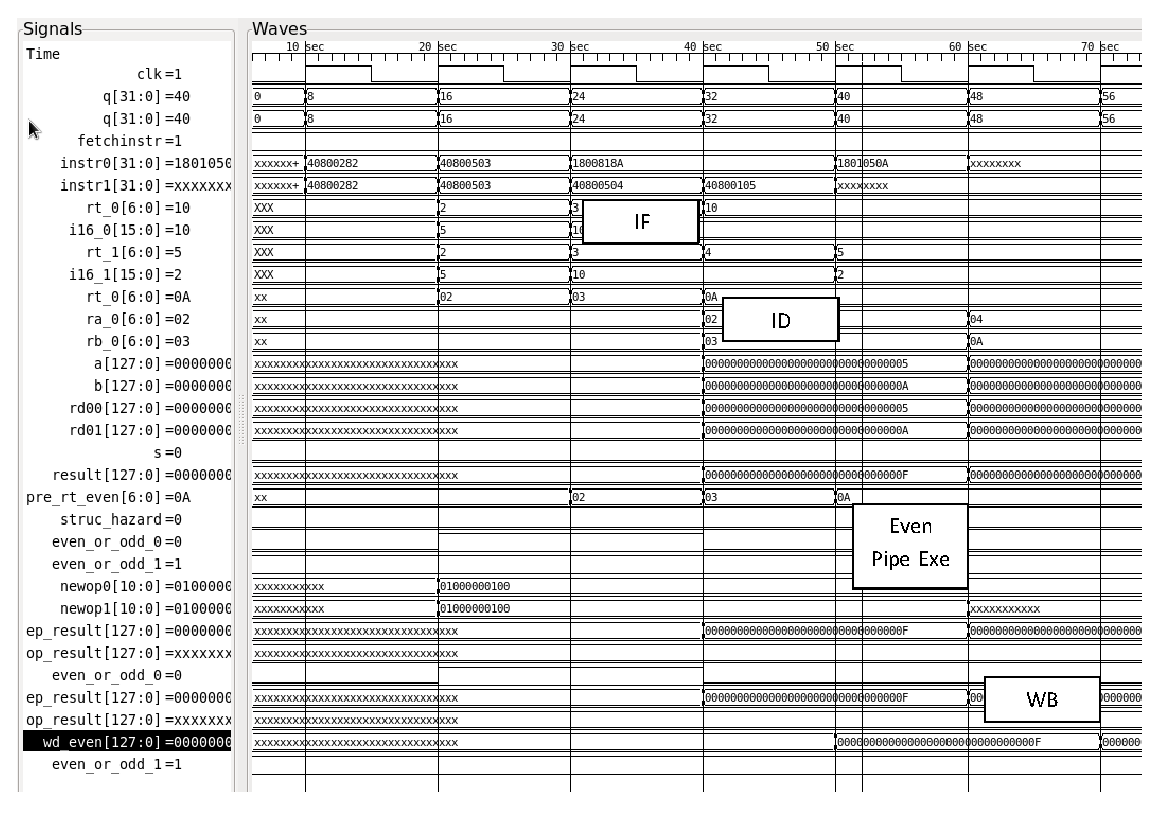
\epsfig{file=test_fig1.eps, width=\textwidth}
\caption{Load immediate and add result}
\label{fig:test_fig1}
\end{figure}


\subsection{Structure Hazard}

Once there is structure hazard, the decoder sends a control signal to
PC alu that the next clock cycle. Then the programm counter's step
becomes to 4 instead of 8. Figure~\ref{fig:test_fig2} shows the change
of programmer counter.

\begin{figure}
\centering
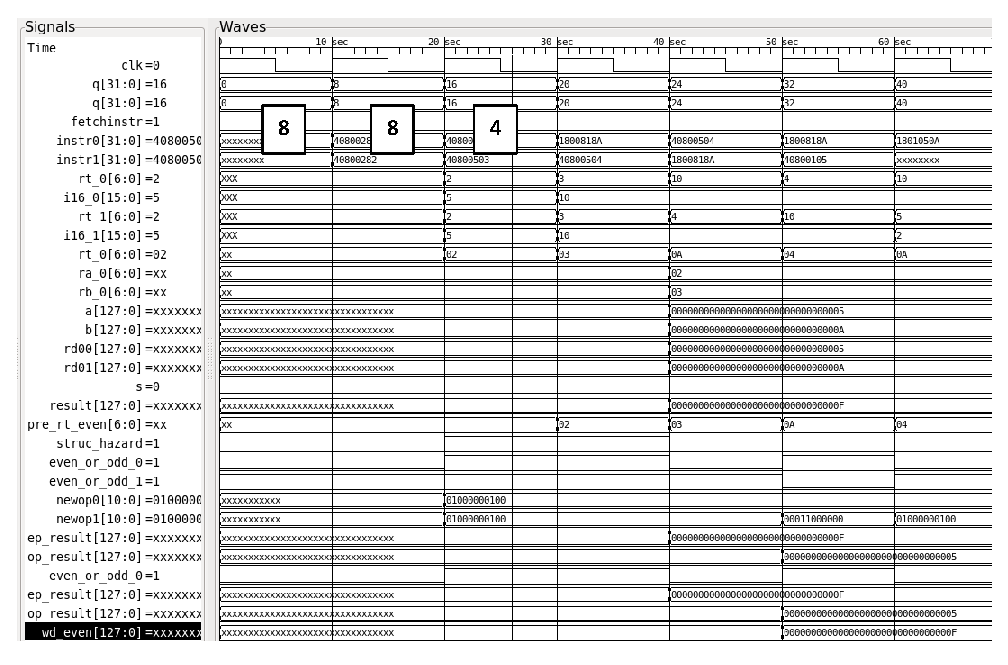
\epsfig{file=test_fig2.eps, width=\textwidth}
\caption{Structual Hazard}
\label{fig:test_fig2}
\end{figure}


\bibliographystyle{model2-names}
\bibliography{rdma}


\end{document}

